%%%%%%%%%%%%%%%%%%%%%%%%%%%%%%%%%%%%%%%%%%%%%%%%%%%%%%%%%%%%%%%%%%%%%%%%%%%%%%%%
\documentclass[10pt,a4paper]{article}
\usepackage[utf8]{inputenc}
\usepackage[T1]{fontenc}
\usepackage{amsmath,amssymb,amsfonts}
\usepackage{geometry}
\usepackage{lmodern}
\usepackage{marvosym}
\usepackage{textcomp}
\DeclareUnicodeCharacter{20AC}{\EUR{}}
\DeclareUnicodeCharacter{2264}{\leqslant}
\DeclareUnicodeCharacter{2265}{\geqslant}
%%=============================================================================
%% Properties

\title{Procedural textures}
\author{\textsc{P.~Neidhardt}}

%%=============================================================================
%% Aliases

\usepackage{xspace}

\let\latexbak\LaTeX
\renewcommand{\LaTeX}{\textrm{\latexbak}\xspace}

\let\texbak\TeX
\renewcommand{\TeX}{\textrm{\texbak}\xspace}

\def\unix{\textsc{Unix}\xspace}
\def\ie{\textsl{i.e.}\xspace}
\def\eg{\textsl{e.g.}\xspace}

%%=============================================================================
%% Formatting

% \usepackage{parskip}
% \setlength{\parindent}{15pt}

% \renewcommand{\thefigure}{\arabic{section}.\arabic{figure}}
\renewcommand{\arraystretch}{1.4}
% \renewcommand{\familydefault}{\sfdefault}

% \usepackage{needspace}

%%==============================================================================
%% Tables

% \usepackage{longtable}
% \usepackage{tabu}

%%==============================================================================
%% Graphics

%% Load TikZ after xcolor.
\usepackage[svgnames]{xcolor}
\usepackage{graphicx}
\usepackage{subfigure}
\graphicspath{{pictures/}}
% \usepackage{tikz}

% \newcommand{\fancybox}[1]{
%   \begin{tikzpicture}
%     \node[draw,rounded corners]{#1};
%   \end{tikzpicture}
% }

%%==============================================================================
%% Misc.

% \usepackage{calc}
% \usepackage{fp}
% \usepackage{lipsum}

%%=============================================================================
%% Listings

% \usepackage{listings}

%% Source code.
% \lstdefinestyle{customc}{
%   % numbers=left,
%   belowcaptionskip=1\baselineskip,
%   breaklines=true,
%   frame=L,
%   xleftmargin=\parindent,
%   % framexleftmargin=\parindent,
%   language=C,
%   showstringspaces=false,
%   basicstyle=\footnotesize\ttfamily,
%   keywordstyle=\bfseries\color{green!40!black},
%   commentstyle=\itshape\color{purple!40!black},
%   identifierstyle=\color{blue},
%   stringstyle=\color{orange},
%   numberstyle=\ttfamily
% }

% \lstset{escapechar=@,style=customc}

%%=============================================================================
%% Babel

%% Load last before 'hyperref'.
%% \usepackage[frenchb]{babel}

%%==============================================================================
%% Hyperref

%% Load last.
\usepackage[]{hyperref}

\hypersetup{
  colorlinks=true,
  linkcolor=DarkRed,
  linktoc=page,
  urlcolor=blue,
}

%%==============================================================================
\newcommand{\definition}[2]{
  \noindent\textbf{#1}\par\vspace{.5\baselineskip}
  \noindent\fbox{
    \begin{minipage}{\textwidth}
      #2
    \end{minipage}
  }
}

\newcommand{\function}[5]{
  \begin{tabular}{rl}
    #1 $\colon$ #2 & $\longrightarrow$ #3 \\
    #4             & $\longmapsto$     #5
  \end{tabular}
}

%%%%%%%%%%%%%%%%%%%%%%%%%%%%%%%%%%%%%%%%%%%%%%%%%%%%%%%%%%%%%%%%%%%%%%%%%%%%%%%%
\begin{document}
%%%%%%%%%%%%%%%%%%%%%%%%%%%%%%%%%%%%%%%%%%%%%%%%%%%%%%%%%%%%%%%%%%%%%%%%%%%%%%%%
\maketitle

\begin{abstract}
  This is a draft on procedural textures.
\end{abstract}

\vfill
\thispagestyle{empty}
\tableofcontents

\section{Interpolation}

\subsection{Linear interpolation}

Linear interpolation function between $a$ and $b$:
\[
\boxed{
  \function {$f$} {$[0;1]$} {$[a;b]$} {$x$} {$a \cdot (1-x) + b \cdot x$}
}
\]

\begin{figure}[p]
  \centering
  \caption{Grayscale linear interpolation}
  \bigskip
  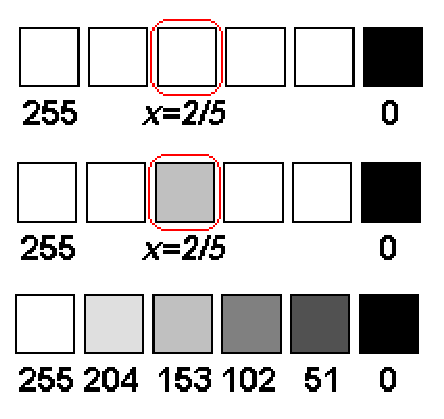
\includegraphics[scale=0.8]{pictures/interpolation}
\end{figure}

%%==============================================================================
\subsection{Bilinear interpolation}

\begin{figure}[p]
  \centering
  \caption{Bilinear interpolation process}
  \bigskip
  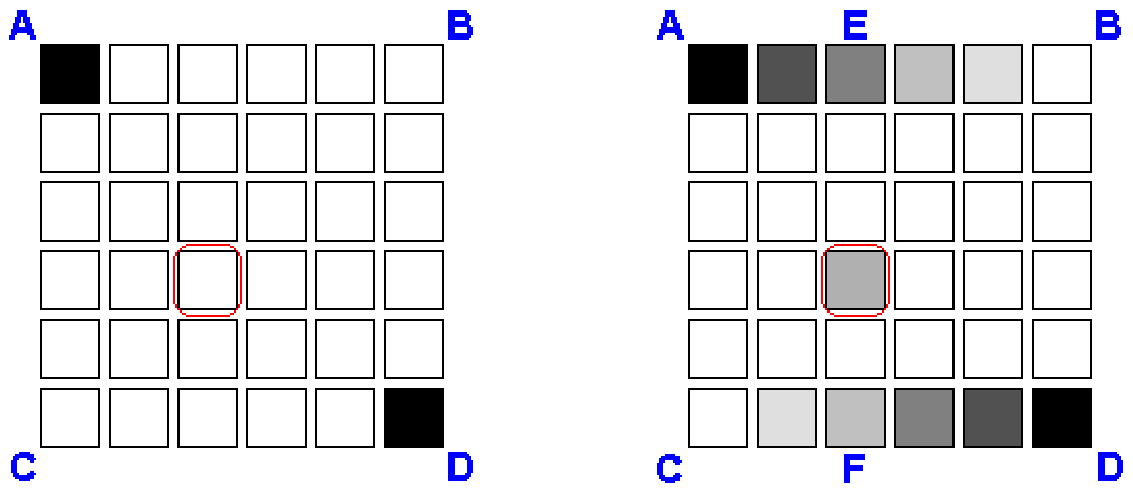
\includegraphics[width=\linewidth]{interpolation_bil}
\end{figure}

\begin{figure}[p]
  \centering
  \caption{Bilinear interpolation}
  \bigskip
  \subfigure[Interpolation points in 2D]{\label{fig:contour-a}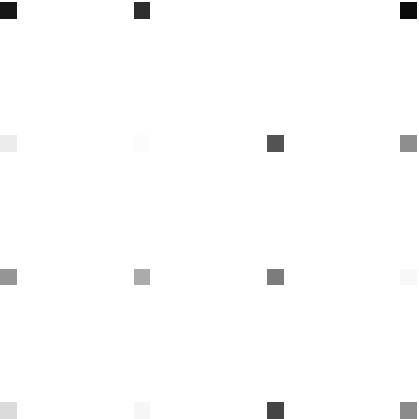
\includegraphics[scale=0.75]{interpol_bil_step1}}
  \subfigure[Applying the bilinear interpolation]{\label{fig:contour-b}
\includegraphics{interpol_bil_step2}}
\end{figure}

%%==============================================================================
\subsubsection{Non-linear interpolation function}

Cosine interpolation between $a$ and $b$:

\[\boxed{
  \function{$f$}{$[0;1]$}{$[a;b]$}{$x$}{$a \cdot \frac {1+\cos(x\cdot\pi)} {2} + b \cdot \frac {1-\cos(x\cdot\pi)} {2}$}
}\]

\begin{figure}[p]
  \centering
  \caption{Cosine interpolation}
  \bigskip
  
\includegraphics{interpol_cos}
\end{figure}

The classic polynomial interpolation is not the fastest. Besides it suffers from
a well-known side-effect called the Runge's phenomenon. Spline functions
(e.g. cubic splines) are faster without any side-effect.

%%==============================================================================
\section{Fusion of various interpolations}

\subsection{Definitions}

\definition{Frequency}{Number of pixels used as interpolation point (on one
  dimension). These pixels are split by a fixed interval called \emph{step},
  which depends on the frequency and the size of the picture.}

\begin{figure}[p]
  \centering
  \caption{Frequency}
  \bigskip
  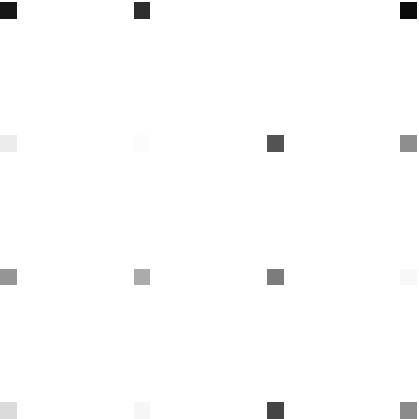
\includegraphics[scale=0.8]{interpol_bil_step1}
\end{figure}

\definition{Octave}{Virtual layer drawn in parallel to the reference layer,
  at a given frequency. Octaves are drawn in sequence, where the $n$th octave
  has a higher frequency than the $n-1$th. A typical increase in frequency would
  be to take the square of the previous value. In the end the resulting layers are merged together.}

\definition{Persistance}{Weight factor for every octave that provides more or
  less impact on the final result.}

\bigskip
Note: since the layer values must reamin in $\{0;255\}$, we must take care that
the sum does not overflow. Limiting the persistence 0.5 makes sure we do not sum
over 255 when octave persistences are powers of the original one.
\[
\sum_{k=1}^{\infty} p^k= \frac {p} {1-p} \leqslant 1 \Rightarrow p \leqslant 0.5
\]

\bigskip
Texture parameters:
\begin{itemize}
\item $\mathbf{ssed} \in \mathbb{N}$
\item $\mathbf{frequency} \in \{ 2^i; i \in \mathbb{N}\}$
\item $\mathbf{octaves} \in \mathbb{N}$
\item $\mathbf{persistence} \in [0,1]$
\end{itemize}


%%%%%%%%%%%%%%%%%%%%%%%%%%%%%%%%%%%%%%%%%%%%%%%%%%%%%%%%%%%%%%%%%%%%%%%%%%%%%%%%
\end{document}
%%%%%%%%%%%%%%%%%%%%%%%%%%%%%%%%%%%%%%%%%%%%%%%%%%%%%%%%%%%%%%%%%%%%%%%%%%%%%%%%

